% Created 2017-05-21 Sun 14:23
% Intended LaTeX compiler: pdflatex
\documentclass[11pt]{article}
\usepackage[utf8]{inputenc}
\usepackage[T1]{fontenc}
\usepackage{graphicx}
\usepackage{grffile}
\usepackage{longtable}
\usepackage{wrapfig}
\usepackage{rotating}
\usepackage[normalem]{ulem}
\usepackage{amsmath}
\usepackage{textcomp}
\usepackage{amssymb}
\usepackage{capt-of}
\usepackage{hyperref}
\usepackage[margin=1.2in]{geometry}
\usepackage{setspace}
\onehalfspacing
\usepackage{parskip}
\usepackage{booktabs}
\usepackage{rotating}
\usepackage{dcolumn}
\newcommand{\pr}{\mathrm{Pr}}
\setcounter{secnumdepth}{1}
\author{Zheng Tian}
\date{\textit{[2016-05-30 Mon]}}
\title{Replication of Examples in Chapter 8: Nonlinear Regression Models}
\hypersetup{
 pdfauthor={Zheng Tian},
 pdftitle={Replication of Examples in Chapter 8: Nonlinear Regression Models},
 pdfkeywords={},
 pdfsubject={},
 pdfcreator={Emacs 25.1.1 (Org mode 9.0.3)},
 pdflang={English}}
\begin{document}

\maketitle


\section{Introduction}
\label{sec:orgd5b8937}

This document shows how to estimate nonlinear regression models. We
will reproduce the estimation results of the application of test
scores in California elementary school districts in Section 8.4 in the
textbook.

The regression concerns the effect of class sizes represented by
student-teacher ratios on test scores. The goals of this regression
are to answer the following research questions:
\begin{enumerate}
\item After controlling for differences in economic characteristics of
different districts, does the effect on test scores of reducing the
student-teacher ratio depend on the fraction of English learners?
\item Does this effect depend on the value of the student-teacher ratio?
\end{enumerate}

\section{Read data}
\label{sec:orga4903c1}

We read the data file, which is \texttt{caschool.dta}.
\begin{verbatim}
library(AER)
# read data
library(foreign)
classdata <- read.dta("./data/caschool.dta")
\end{verbatim}

The regression models in this application involve the dependent
variable of test scores (\emph{TestScore}), and various independent variables, including
the student-teacher ratio (\emph{STR}), the percentage of English learners
(\emph{PctEL}), the percentage of students eligible for subsidized lunch
(\emph{PctLch}), and average district income (\emph{Income}). The corresponding
variables in \texttt{classdata} are \texttt{str}, \texttt{el\_pct}, \texttt{meal\_pct}, and
\texttt{avginc}.

We first get basic descriptive statistics of these variables.
\begin{verbatim}
var2use <- c("testscr", "str", "el_pct", "meal_pct", "avginc")
df2use <- classdata[var2use]
sumdf <- summary(df2use)
\end{verbatim}

Usually, we present these descriptive statistics in a table. We can
use the function of \texttt{stargazer} to generate Table \ref{tab:destab}.
\begin{verbatim}
varlabs <- c(
    "Average test scores",
    "Student-teacher ratio",
    "Percent of English learners",
    "Percent of students eligible for subsidized lunch",
    "Average district income"
)

library(stargazer)
stargazer(df2use, title = "Descriptive Statistics of All Variables",
	  covariate.labels = varlabs,
	  summary.stat = c("max", "mean", "median", "min", "sd"),
	  digits = 2,
	  label = "tab:destab"
)
\end{verbatim}


% Table created by stargazer v.5.2 by Marek Hlavac, Harvard University. E-mail: hlavac at fas.harvard.edu
% Date and time: Sun, May 21, 2017 - 14:23:34
\begin{table}[!htbp] \centering
  \caption{Descriptive Statistics of All Variables}
  \label{tab:destab}
\begin{tabular}{@{\extracolsep{5pt}}lccccc}
\\[-1.8ex]\hline
\hline \\[-1.8ex]
Statistic & \multicolumn{1}{c}{Max} & \multicolumn{1}{c}{Mean} & \multicolumn{1}{c}{Median} & \multicolumn{1}{c}{Min} & \multicolumn{1}{c}{St. Dev.} \\
\hline \\[-1.8ex]
Average test scores & 706.75 & 654.16 & 654.45 & 605.55 & 19.05 \\
Student-teacher ratio & 25.80 & 19.64 & 19.72 & 14.00 & 1.89 \\
Percent of English learners & 85.54 & 15.77 & 8.78 & 0.00 & 18.29 \\
Percent of students eligible for subsidized lunch & 100.00 & 44.71 & 41.75 & 0.00 & 27.12 \\
Average district income & 55.33 & 15.32 & 13.73 & 5.34 & 7.23 \\
\hline \\[-1.8ex]
\end{tabular}
\end{table}

Finally, we can generate a scatterplot to visualize the relationship
between test scores and student-teacher ratios.

\begin{verbatim}
plot(testscr ~ str, data = df2use,
     main = "The scatterplot of test scores against student-teacher ratios",
     xlab = "Student-teacher ratio", ylab = "Test scores",
     bty = "l", col = "blue")
\end{verbatim}

\begin{figure}[htbp]
\centering
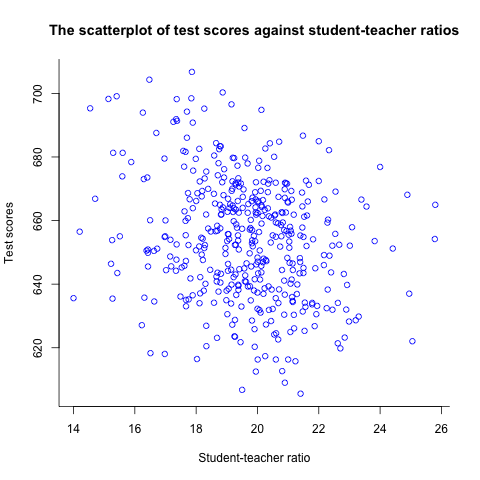
\includegraphics[width=0.85\textwidth]{img/scplot.png}
\caption{The scatterplot of test scores and student-teacher ratios}
\end{figure}

\section{Regression models}
\label{sec:org215456b}
We estimate seven regression models that appear in Table 8.3 in
Chapter 8 of the textbook.

\subsection*{Create a binary variable \emph{HiEL}}
\label{sec:org1c4f719}

Since some regressions in this table use
the independent variable of \emph{HiEL} that is a binary variable for the
districts with the percentage of English learners higher than 10\%, we
first need to generate such variable.

\begin{verbatim}
hiel <- ifelse(df2use$el_pct > 10, TRUE, FALSE)
table(hiel)
\end{verbatim}

\begin{center}
\begin{tabular}{lr}
FALSE & 228\\
TRUE & 192\\
\end{tabular}
\end{center}

We can see that there are 370 districts categorized as having high
percentage of English learners.

\subsection*{Set up regression models}
\label{sec:org8e79bc6}

We need to set up seven regression models as follows:
\begin{verbatim}
fm1 <- testscr ~ str + el_pct + meal_pct
fm2 <- testscr ~ str + el_pct + meal_pct + log(avginc)
fm3 <- testscr ~ hiel*str
fm4 <- testscr ~ hiel*str + meal_pct + log(avginc)
fm5 <- testscr ~ str + I(str^2) + I(str^3) + hiel + meal_pct + log(avginc)
fm6 <- testscr ~ hiel*str + hiel*I(str^2) + hiel*I(str^3) + meal_pct + log(avginc)
fm7 <- testscr ~ str + I(str^2) + I(str^3) + el_pct + meal_pct + log(avginc)
\end{verbatim}

Since they are all linear with respect to the parameters, we can
estimate them using OLS with the function \texttt{lm()} one by one. However,
writing the commands of \texttt{lm()} for each specification is repetitive
work, which is more easily done with a loop. Of course, we can use
\texttt{for} loop to do so, but R has a family of \texttt{apply()} functions that make
running a loop much easier. Here we use the \texttt{lapply()} function.

\texttt{lapply()} takes its first argument as a \texttt{list} object, and the second
argument as the name of a function that is imposed on each item in the
\texttt{list} object, and the third or more arguments as the other inputs for
that function. Before using \texttt{lapply}, we use the \texttt{mget()} function to
generate a \texttt{list} object consisting of all formula specified
above. Also, we define a function of \texttt{allols()} that wraps the \texttt{lm()}
function, using the default data set of \texttt{df2use}. Finally, \texttt{lapply()}
returns a \texttt{list} object consisting of all the \texttt{lm} objects estimated
by the \texttt{lm()} function.

\begin{verbatim}
fm.ls <- mget(paste("fm", 1:7, sep = ""))
allols <- function(x) lm(x, data = df2use)
ols.all <- lapply(fm.ls, allols)
\end{verbatim}

We present all estimation results in Table \ref{tab:tab83} using the
\texttt{stargazer} function. Since this function reports the homoskedasticity-only
standard errors of the coefficients by default, we need to replace
them with the heteroskedasticity-robust standard errors.

\begin{verbatim}
coef.all <- lapply(ols.all, coef)
hccm.all <- lapply(ols.all, vcovHC, type = "HC1")
seht.all <- lapply(hccm.all, function(x) sqrt(diag(x)))

indep.labels <- c("$STR$", "$STR^2$", "$STR^3$",
		  "Percent of English learner",
		  "High Percent of English learner",
		  "$HiEL \\times STR$", "$HiEL \\times STR^2$",
		  "$HiEL \\times STR^3$", "Percent of eligible for free lunch",
		  "Average district income")

stargazer(ols.all, title = "Nonlinear regression models of test scores",
	  coef = coef.all, se = seht.all,
	  covariate.labels = indep.labels,
	  dep.var.caption = "Dependent variable: Average test scores",
	  dep.var.labels.include = FALSE,
	  no.space = TRUE, df = FALSE,
	  order = c(2, 4, 5, 3, 1, 8, 9, 10, 6, 7, 11),
	  float.env = "sidewaystable",
	  label = "tab:tab83")
\end{verbatim}


% Table created by stargazer v.5.2 by Marek Hlavac, Harvard University. E-mail: hlavac at fas.harvard.edu
% Date and time: Sun, May 21, 2017 - 14:23:35
% Requires LaTeX packages: rotating
\begin{sidewaystable}[!htbp] \centering
  \caption{Nonlinear regression models of test scores}
  \label{tab:tab83}
\begin{tabular}{@{\extracolsep{5pt}}lccccccc}
\\[-1.8ex]\hline
\hline \\[-1.8ex]
 & \multicolumn{7}{c}{Dependent variable: Average test scores} \\
\cline{2-8}
\\[-1.8ex] & (1) & (2) & (3) & (4) & (5) & (6) & (7)\\
\hline \\[-1.8ex]
 $STR$ & $-$0.998$^{***}$ & $-$0.734$^{***}$ & $-$0.968 & $-$0.531 & 64.339$^{***}$ & 83.701$^{***}$ & 65.285$^{***}$ \\
  & (0.270) & (0.257) & (0.589) & (0.342) & (24.861) & (28.497) & (25.259) \\
  $STR^2$ &  &  &  &  & $-$3.424$^{***}$ & $-$4.381$^{***}$ & $-$3.466$^{***}$ \\
  &  &  &  &  & (1.250) & (1.441) & (1.271) \\
  $STR^3$ &  &  &  &  & 0.059$^{***}$ & 0.075$^{***}$ & 0.060$^{***}$ \\
  &  &  &  &  & (0.021) & (0.024) & (0.021) \\
  Percent of English learner & $-$0.122$^{***}$ & $-$0.176$^{***}$ &  &  &  &  & $-$0.166$^{***}$ \\
  & (0.033) & (0.034) &  &  &  &  & (0.034) \\
  High Percent of English learner &  &  & 5.639 & 5.498 & $-$5.474$^{***}$ & 816.075$^{**}$ &  \\
  &  &  & (19.515) & (9.795) & (1.034) & (327.674) &  \\
  $HiEL \times STR$ &  &  & $-$1.277 & $-$0.578 &  & $-$123.282$^{**}$ &  \\
  &  &  & (0.967) & (0.496) &  & (50.213) &  \\
  $HiEL \times STR^2$ &  &  &  &  &  & 6.121$^{**}$ &  \\
  &  &  &  &  &  & (2.542) &  \\
  $HiEL \times STR^3$ &  &  &  &  &  & $-$0.101$^{**}$ &  \\
  &  &  &  &  &  & (0.043) &  \\
  Percent of eligible for free lunch & $-$0.547$^{***}$ & $-$0.398$^{***}$ &  & $-$0.411$^{***}$ & $-$0.420$^{***}$ & $-$0.418$^{***}$ & $-$0.402$^{***}$ \\
  & (0.024) & (0.033) &  & (0.029) & (0.029) & (0.029) & (0.033) \\
  Average district income &  & 11.569$^{***}$ &  & 12.124$^{***}$ & 11.748$^{***}$ & 11.800$^{***}$ & 11.509$^{***}$ \\
  &  & (1.819) &  & (1.798) & (1.771) & (1.778) & (1.806) \\
  Constant & 700.150$^{***}$ & 658.552$^{***}$ & 682.246$^{***}$ & 653.666$^{***}$ & 252.051 & 122.354 & 244.809 \\
  & (5.568) & (8.642) & (11.868) & (9.869) & (163.634) & (185.519) & (165.722) \\
 \hline \\[-1.8ex]
Observations & 420 & 420 & 420 & 420 & 420 & 420 & 420 \\
R$^{2}$ & 0.775 & 0.796 & 0.310 & 0.797 & 0.801 & 0.803 & 0.801 \\
Adjusted R$^{2}$ & 0.773 & 0.794 & 0.305 & 0.795 & 0.798 & 0.799 & 0.798 \\
Residual Std. Error & 9.080 & 8.643 & 15.880 & 8.629 & 8.559 & 8.547 & 8.568 \\
F Statistic & 476.306$^{***}$ & 405.359$^{***}$ & 62.399$^{***}$ & 325.804$^{***}$ & 277.212$^{***}$ & 185.777$^{***}$ & 276.515$^{***}$ \\
\hline
\hline \\[-1.8ex]
\textit{Note:}  & \multicolumn{7}{r}{$^{*}$p$<$0.1; $^{**}$p$<$0.05; $^{***}$p$<$0.01} \\
\end{tabular}
\end{sidewaystable}

\section{Discussion of the results}
\label{sec:org93c8c99}
\subsection*{The research questions}
\label{sec:org712d216}
Keep in mind that we have two research questions to answer:
\begin{enumerate}
\item Does this effect depend on the value of the student-teacher ratio?
\item After controlling for differences in economic characteristics of
different districts, does the effect on test scores of reducing the
student-teacher ratio depend on the fraction of English learners?
\end{enumerate}
\subsection*{The polynomial terms of \emph{STR}}
\label{sec:org97e04e0}
Regression models (5), (6), and (7) include the polynomial terms of
\emph{STR}. The t-statistics for all these coefficients on \(STR\), \(STR^2\),
and \(STR^3\) are greater than the critical value of the normal
distribution at the 1\% level. Thus, they are all statistically
significant individually.

The joint zero hypotheses for \(STR^2\) and \(STR^3\) can be tested using
the F-statistics for all the three regression models.

\begin{verbatim}
testSTR23 <- function(ols.res, vcov.hc){
    test <- linearHypothesis(ols.res, c("I(str^2) = 0", "I(str^3) = 0"),
			     vcov. = vcov.hc)
    fstat <- test[2, 3]
    pval <- test[2, 4]
    return(list(Fstat = fstat, Pval = pval, Test = test))
}

F5 <- testSTR23(ols.all[[5]], hccm.all[[5]])
F6 <- testSTR23(ols.all[[6]], hccm.all[[6]])
F7 <- testSTR23(ols.all[[7]], hccm.all[[7]])
\end{verbatim}

The F statistics and their corresponding p-values are
\begin{itemize}
\item Regression (5): The F-statistic is \texttt{6.17} with
the p-value of \texttt{0.0023};
\item Regression (6): The F-statistic is \texttt{5.81} with
the p-value of \texttt{0.0033};
\item Regression (7): The F-statistic is \texttt{5.96} with
the p-value of \texttt{0.0028}.
\end{itemize}
Therefore, the joint zero hypotheses are rejected for all three models
at the 1\% level. That means that there is nonlinear effect of \emph{STR} on
test scores.

The simplest way to interpret the nonlinear effect of \emph{STR} on test
scores is by plotting the estimated regression lines. To generate the
estimated regression lines, we need to get the predicted values of test
scores based on a range of the values of \emph{STR}, holding other variable
constant. Except for \emph{STR}, we let all the continuous variables take
their average values and let \emph{HiEL} be one. \emph{STR} takes the values
from its minimum value to its maximum value, with a step of 0.05.

The following codes get the predicted values of test scores and draw
the regression lines.
\begin{verbatim}
str.sim <- with(df2use, seq(min(str), max(str), by = 0.05))
n.sim <- length(str.sim)
means <- lapply(df2use, mean)
means$hiel <- ifelse(mean(hiel) > 0.5, TRUE, FALSE)
newdf <- data.frame(str = str.sim,
		    el_pct = rep(means$el_pct, n.sim),
		    meal_pct = rep(means$meal_pct, n.sim),
		    avginc = rep(means$avginc, n.sim),
		    hiel = rep(means$hiel, n.sim))

yhat.2 <- predict(ols.all[[2]], newdata = newdf)
yhat.5 <- predict(ols.all[[5]], newdata = newdf)
yhat.7 <- predict(ols.all[[7]], newdata = newdf)

plot(testscr ~ str, data = df2use,
     xlab = "Student-teacher ratio", ylab = "Test scores",
     bty = "l", col = "gray")
lines(yhat.2 ~ str.sim, col = "black", lwd = 1.5)
lines(yhat.5 ~ str.sim, col = "red", lwd = 1.5)
lines(yhat.7 ~ str.sim, col = "blue", lty = 2, lwd = 1.5)
legend("topright", c("Linear regression (2)",
		     "Cubic regression (5)",
		     "Cubic regression (7)"),
       col = c("black", "red", "blue"),
       lty = c(1, 1, 2))
\end{verbatim}

\begin{figure}[htbp]
\centering
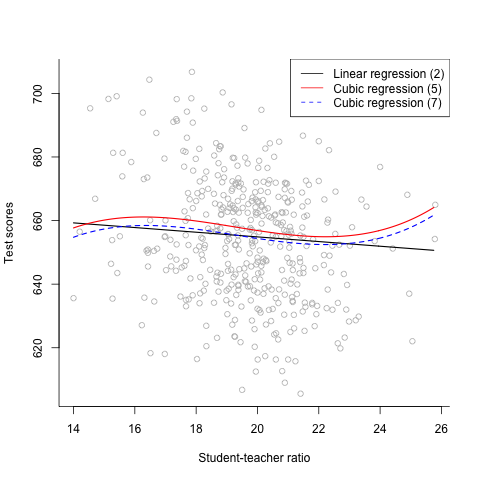
\includegraphics[width=0.85\textwidth]{./img/fig-8-10.png}
\caption{\label{fig:org9c90b99}
Three regression lines relating test scores and student-teacher ratios}
\end{figure}

\subsection*{The interaction between \emph{STR} and \emph{HiEL}}
\label{sec:orgfbce228}
Regression models (3), (4), and (6) include the interaction terms of
\emph{STR} and \emph{HiEL}. Regressions (3) and (4) only have the interaction
term of \emph{HiEL} and \emph{STR}, which is neither significant at the 10\%
level, while Regression (6) has the interaction terms of \emph{HiEL} and
\(STR\), \(STR^2\), and \(STR^3\), which are individually significant at the
5\% level. The joint hypothesis of all the interaction terms having
zero coefficients can be tested as follows
\begin{verbatim}
F6.inter <- linearHypothesis(ols.all[[6]],
			     c("hielTRUE:str=0", "hielTRUE:I(str^2)=0",
			       "hielTRUE:I(str^3)=0"), vcov. = hccm.all[[6]])
\end{verbatim}

The F-statistic is \texttt{2.69} with the p-value of
\texttt{0.046} so that the coefficients on the three
interaction terms are jointly significant at the 5\% level but
insignificant at the 1\% level.

Also, we can plot the regression lines in Regression (6) for \(HiEL=1\)
and \(HiEL=0\).

\begin{verbatim}
# plot Figure 8.11
df2use.a <- df2use[hiel, ]
df2use.b <- df2use[!hiel, ]

newdf$hiel <- TRUE
yhat.6.T <- predict(ols.all[[6]], newdata = newdf)

newdf$hiel <- FALSE
yhat.6.F <- predict(ols.all[[6]], newdata = newdf)

plot(testscr ~ str, data = df2use.a,
     xlab = "Student-teacher ratio", ylab = "Test scores",
     bty = "l", col = "gray")
points(testscr ~ str, data = df2use.b, col = "orange")
lines(yhat.6.T ~ str.sim, col = "blue", lwd = 1.5)
lines(yhat.6.F ~ str.sim, col = "red", lwd = 1.5, lty = 2)
legend("topright", legend = c("High EL", "Low EL"),
       pch = c(1, 1), col = c("gray", "orange"))
legend(18, 615, legend = c("Regression with HiEL=1",
				 "Regression with HiEL = 0"),
       col = c("blue", "red"), lty = c(1, 2))
\end{verbatim}

\begin{figure}[htbp]
\centering
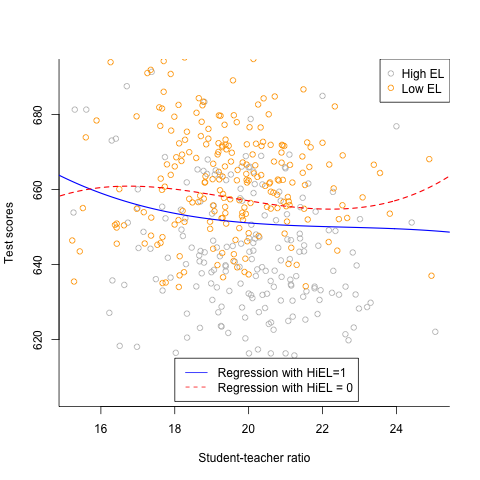
\includegraphics[width=0.85\textwidth]{./img/fig-8-11.png}
\caption{\label{fig:org97997ac}
The regression lines for districts with high and low percentage of English learners}
\end{figure}

\subsection*{Conclusion}
\label{sec:orgd12ec1e}
\section{Appendix: R codes}
\label{sec:orgddd1dbf}
\begin{verbatim}
# read the data files into R
# read the dta file
library(AER)

library(foreign)
classdata <- read.dta("./data/caschool.dta")

# extract variables used in regression models
var2use <- c("testscr", "str", "el_pct", "meal_pct", "avginc")
df2use <- classdata[var2use]

## descriptive statistics
sumdf <- summary(df2use)

varlabs <- c(
    "Average test scores",
    "Student-teacher ratio",
    "Percent of English learners",
    "Percent eligible for subsidized lunch",
    "Average district income"
)

library(stargazer)
stargazer(df2use, title = "Descriptive Statistics of All Variables",
          covariate.labels = varlabs,
          summary.stat = c("max", "mean", "median", "min", "sd"),
          digits = 2,
          label = "tab:destab"
)

plot(testscr ~ str, data = df2use,
     main = "The scatterplot of test scores against student-teacher ratios",
     xlab = "Student-teacher ratio", ylab = "Test scores",
     bty = "l", col = "blue")

## regressions

hiel <- ifelse(df2use$el_pct > 10, TRUE, FALSE)
table(hiel)

fm1 <- testscr ~ str + el_pct + meal_pct
fm2 <- testscr ~ str + el_pct + meal_pct + log(avginc)
fm3 <- testscr ~ str + hiel + hiel:str
fm4 <- testscr ~ str + hiel + hiel:str + meal_pct + log(avginc)
fm5 <- testscr ~ str + I(str^2) + I(str^3) + hiel + meal_pct + log(avginc)
fm6 <- testscr ~ hiel*str + hiel*I(str^2) + hiel*I(str^3) + meal_pct + log(avginc)
fm7 <- testscr ~ str + I(str^2) + I(str^3) + el_pct + meal_pct + log(avginc)

fm.ls <- mget(paste("fm", 1:7, sep = ""))

allols <- function(x) lm(x, data = df2use)
ols.all <- lapply(fm.ls, allols)

coef.all <- lapply(ols.all, coef)
hccm.all <- lapply(ols.all, vcovHC, type = "HC1")
seht.all <- lapply(hccm.all, function(x) sqrt(diag(x)))

indep.labels <- c("$STR$", "$STR^2$", "$STR^3$",
                  "Percent of English learner",
                  "High Percent of English learner",
                  "$HiEL \\times STR$", "$HiEL \\times STR^2$",
                  "$HiEL \\times STR^3$", "Percent of eligible for free lunch",
                  "Average district income")

stargazer(ols.all, title = "Nonlinear regression models of test scores",
          coef = coef.all, se = seht.all,
          covariate.labels = indep.labels,
          dep.var.caption = "Dependent variable: Average test scores",
          dep.var.labels.include = FALSE,
          no.space = TRUE, df = FALSE,
          order = c(2, 4, 5, 3, 1, 8, 9, 10, 6, 7, 11),
          label = "tab:tab83")


# Hypothesis tests
# STR^2 and STR^3

testSTR23 <- function(ols.res, vcov.hc){
    test <- linearHypothesis(ols.res, c("I(str^2) = 0", "I(str^3) = 0"),
                             vcov. = vcov.hc)
    fstat <- test[2, 3]
    pval <- test[2, 4]
    return(list(Fstat = fstat, Pval = pval, Test = test))
}

F5 <- testSTR23(ols.all[[5]], hccm.all[[5]])
F6 <- testSTR23(ols.all[[6]], hccm.all[[6]])
F7 <- testSTR23(ols.all[[7]], hccm.all[[7]])

# plotting
# Plot Figure 8.10
str.sim <- with(df2use, seq(min(str), max(str), by = 0.05))
n.sim <- length(str.sim)
means <- lapply(df2use, mean)
means$hiel <- ifelse(mean(hiel) > 0.5, TRUE, FALSE)
newdf <- data.frame(str = str.sim,
                    el_pct = rep(means$el_pct, n.sim),
                    meal_pct = rep(means$meal_pct, n.sim),
                    avginc = rep(means$avginc, n.sim),
                    hiel = rep(means$hiel, n.sim))

yhat.2 <- predict(ols.all[[2]], newdata = newdf)
yhat.5 <- predict(ols.all[[5]], newdata = newdf)
yhat.7 <- predict(ols.all[[7]], newdata = newdf)

F6.inter <- linearHypothesis(ols.all[[6]],
                             c("hielTRUE:str=0", "hielTRUE:I(str^2)=0",
                               "hielTRUE:I(str^3)=0"), vcov. = hccm.all[[6]])


plot(testscr ~ str, data = df2use,
     xlab = "Student-teacher ratio", ylab = "Test scores",
     bty = "l", col = "gray")
lines(yhat.2 ~ str.sim, col = "black", lwd = 1.5)
lines(yhat.5 ~ str.sim, col = "red", lwd = 1.5)
lines(yhat.7 ~ str.sim, col = "blue", lty = 2, lwd = 1.5)
legend("topright", c("Linear regression (2)",
                     "Cubic regression (5)",
                     "Cubic regression (7)"),
       col = c("black", "red", "blue"),
       lty = c(1, 1, 2))

# plot Figure 8.11
df2use.a <- df2use[hiel, ]
df2use.b <- df2use[!hiel, ]

newdf$hiel <- TRUE
yhat.6.T <- predict(ols.all[[6]], newdata = newdf)

newdf$hiel <- FALSE
yhat.6.F <- predict(ols.all[[6]], newdata = newdf)

plot(testscr ~ str, data = df2use.a,
     xlab = "Student-teacher ratio", ylab = "Test scores",
     bty = "l", col = "gray")
points(testscr ~ str, data = df2use.b, col = "orange")
lines(yhat.6.T ~ str.sim, col = "blue", lwd = 1.5)
lines(yhat.6.F ~ str.sim, col = "red", lwd = 1.5, lty = 2)
legend("topright", legend = c("High EL", "Low EL"),
       pch = c(1, 1), col = c("gray", "orange"))
legend(18, 615, legend = c("Regression with HiEL=1",
                           "Regression with HiEL = 0"),
       col = c("blue", "red"), lty = c(1, 2))
\end{verbatim}
\end{document}